\documentclass{assets/utmreport}

\usepackage{booktabs,amssymb,float,graphicx,listings}

\hypersetup{hidelinks,hypertexnames=false,pdfauthor={Lucian-Adrian Gavril}}

\selectlanguage{english}

\utmlogo{assets/utm-logo.jpeg}

\institution{Technical University of Moldova}
\faculty{Faculty of Computers, Informatics, and Microelectronics}
\department{Department of Software Engineering}
\studyprogramme{Software Engineering Study Programme}
\documenttype{Laboratory report}
\reporttitle{Operating Systems Laboratory 7}
\reportsubtitle{Three Small Programs: Processes, Redirection and a Pipe}
\student{Lucian-Adrian Gavril}{FAF-241}
\supervisor{Reițman Patricia}{univ. assist.}
\cityyear{Chișinău}{2026}

\setlength{\emergencystretch}{3em}
\lstset{basicstyle=\ttfamily\fontsize{10}{12}\selectfont,breaklines=true,columns=fullflexible,keepspaces=true,showstringspaces=false,numbers=left,numberstyle=\tiny\color{gray},frame=single,rulecolor=\color{gray},tabsize=2}

\begin{document}
\makeutmreporttitlepage
\tableofcontents
\clearpage
\begin{utmabstract}[Abstract]
This laboratory reconstructs shell command execution using Linux process and descriptor calls. Four programs demonstrate fork/exec/wait, a visible zombie, file redirection and a two-process pipeline. An optional three-process pipeline extends the same wiring. Observations under Ubuntu 24.04 WSL2 show the expected exit statuses, descriptor allocation and matching shell pipeline counts. A retained write-end reference explains the intentionally blocked consumer.
\utmkeywords{processes, system calls, file descriptors, pipes, linux, xv6}
\end{utmabstract}
\utmintroduction
The required experiments follow the laboratory handout\cite{brief}; the process and descriptor model follows the course lecture\cite{lecture}. The supplied source is reproduced in Appendix A. A successful execution is evidence for that captured environment, while the concept figures explain the general mechanism.

The UNIX process interface lets a shell compose small programs without changing their implementations. Process calls control which program runs and when its completion is collected; file descriptors select where the program reads and writes. These mechanisms explain redirection, pipelines and communication between processes.
This lab reconstructs shell command execution in C. Four programs exercise process creation and replacement, child reaping, output redirection and a two-stage pipeline. A three-stage pipeline extends the same descriptor-wiring mechanism.


\textbf{Measured environment:} Ubuntu 24.04 under WSL2, kernel \texttt{6.\allowbreak{}18.\allowbreak{}33.\allowbreak{}2-\allowbreak{}microsoft-\allowbreak{}standard-\allowbreak{}WSL2}, GCC \texttt{13.\allowbreak{}3.\allowbreak{}0}. The 19 October 2026 capture session compiled all five programs with \texttt{gcc -\allowbreak{}Wall -\allowbreak{}Wextra}.


\chapter{Part 1: \texttt{fork}, \texttt{exec} and \texttt{wait}}
Figure~\ref{fig:lifetime} distinguishes a new process from a replacement program. The amber interval represents an exited child retained until its parent reaps it; the child executes no instructions in that interval.

\begin{figure}[htbp]
\centering
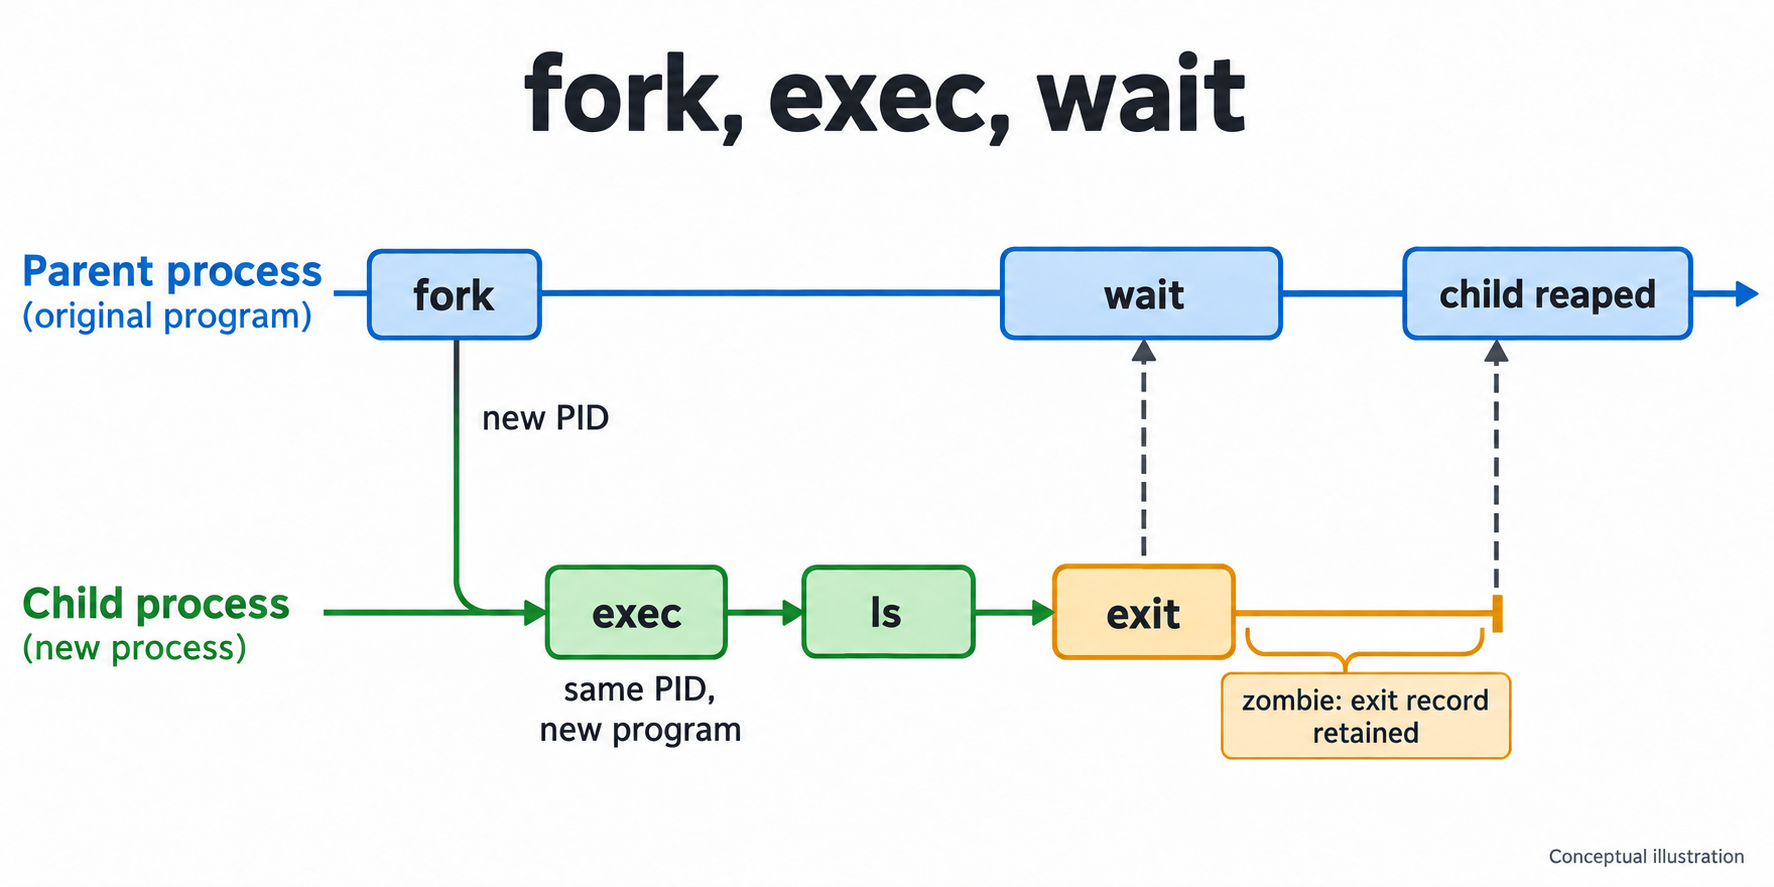
\includegraphics[width=\textwidth]{assets/concept-process-lifetime.png}
\caption{Process lifetime and the retained exit record. ImageGen concept illustration, 23 October 2026; scheduling is schematic.}
\label{fig:lifetime}
\end{figure}


The related xv6 implementation can be compared in the course source snapshot\cite{xv6}. A program is stored instructions; a process is a running instance with an address space, registers and open descriptors. A successful \texttt{fork} creates a child and returns twice: zero in the child and the child PID in the parent. Their relative scheduling is not fixed. In this program the parent waits, which puts its completion message after the child has finished.

The child calls \texttt{execlp} to replace its program with \texttt{ls}. Successful replacement keeps the PID, but changes the program image. It never returns to the old child code. The parent remains in \texttt{run} and collects the child's status with \texttt{waitpid}. Linux encodes the termination information in the status word; \texttt{WEXITSTATUS} is meaningful for normal termination. The supplied example assumes that path; general code also checks \texttt{WIFEXITED}.


\begin{figure}[htbp]
\centering
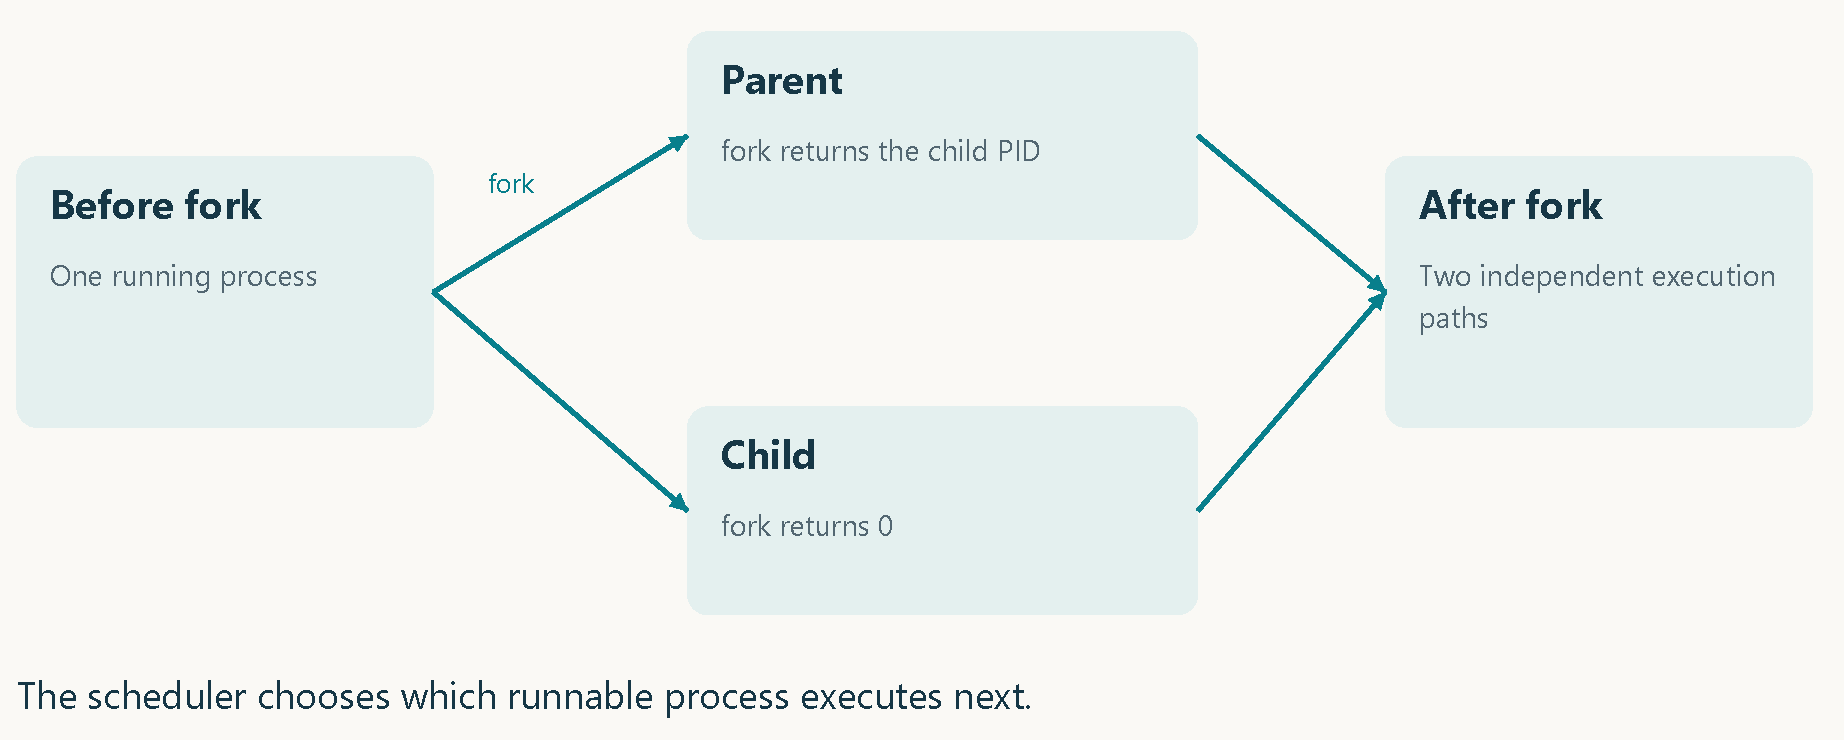
\includegraphics[width=\textwidth]{assets/process-flow.pdf}
\caption{fork creates two execution paths. The parent and child distinguish their paths by the return value.}
\end{figure}


\section{Observe 1}

\textbf{Measured:} The canonical \texttt{ls} child exited with status \texttt{0}; the temporary \texttt{date} child also exited with status \texttt{0}. Neither successful execution printed the \texttt{perror("exec")} message. With \texttt{nosuchprog}, the child printed \texttt{exec: No such file or directory} and the parent reported exit status \texttt{127}.


\textbf{Explanation:} A successful \texttt{execlp} replaces the child's program image and does not return to the old code, so execution never reaches \texttt{perror}. When the requested program is missing, \texttt{execlp} returns with an error; the next line reports it, and the child exits with \texttt{127}.


\section{Observe 2}

\textbf{Measured:} The parent printed PID \texttt{1795}; the child printed its parent PID as \texttt{1795} and its own PID as \texttt{1796}.


\textbf{Explanation:} \texttt{getppid()} returns the PID of the process that created this child. The parent stays alive in \texttt{waitpid}, so its identity has not changed before the child prints.


\section{Observe 3}

\textbf{Measured:} The parent reported status \texttt{0} for \texttt{ls} and \texttt{127} for \texttt{nosuchprog}. The \texttt{date} variant reported status \texttt{0} as well.


\textbf{Explanation:} The \texttt{ls} program exited successfully with status \texttt{0}. The failed-\texttt{exec} branch explicitly calls \texttt{exit(127)}. \texttt{waitpid} collects that child's status for the parent.



\begin{figure}[H]
\centering
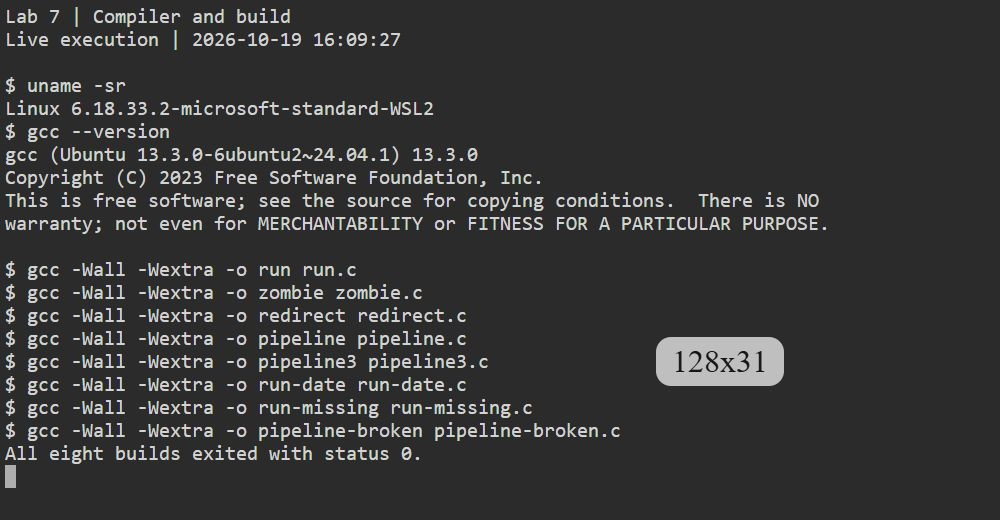
\includegraphics[trim=0bp 14.00bp 0.00bp 0bp,clip,width=\textwidth,height=0.72\textheight,keepaspectratio]{assets/proof-build.png}
\caption{Live Linux console: GCC version and successful builds with -Wall -Wextra. Live ttyd terminal capture, 19 October 2026. Only blank margins are cropped in this report; program output is unchanged.}
\end{figure}


\begin{figure}[H]
\centering
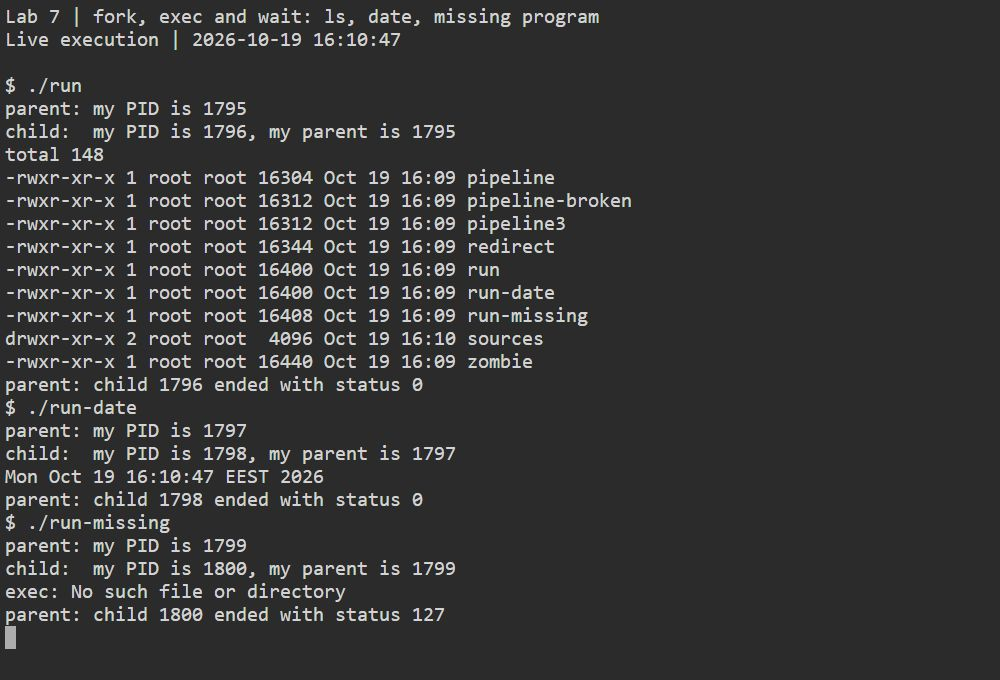
\includegraphics[trim=0bp 13.00bp 0.00bp 0bp,clip,width=\textwidth,height=0.72\textheight,keepaspectratio]{assets/proof-exec.png}
\caption{Live Linux console: the ls and date replacements succeed; the missing-command branch reports exit status 127. Live ttyd terminal capture, 19 October 2026. Only blank margins are cropped in this report; program output is unchanged.}
\end{figure}


\chapter{Part 2: a zombie}

When a child exits, it stops executing and releases its ordinary execution resources. The kernel retains the PID and completion information until its parent collects them. This exited, unreaped state is called a zombie. It differs from a running orphan whose parent has exited. Delaying the parent's wait exposes the zombie; sleeping does not itself reap the child.


\begin{figure}[htbp]
\centering
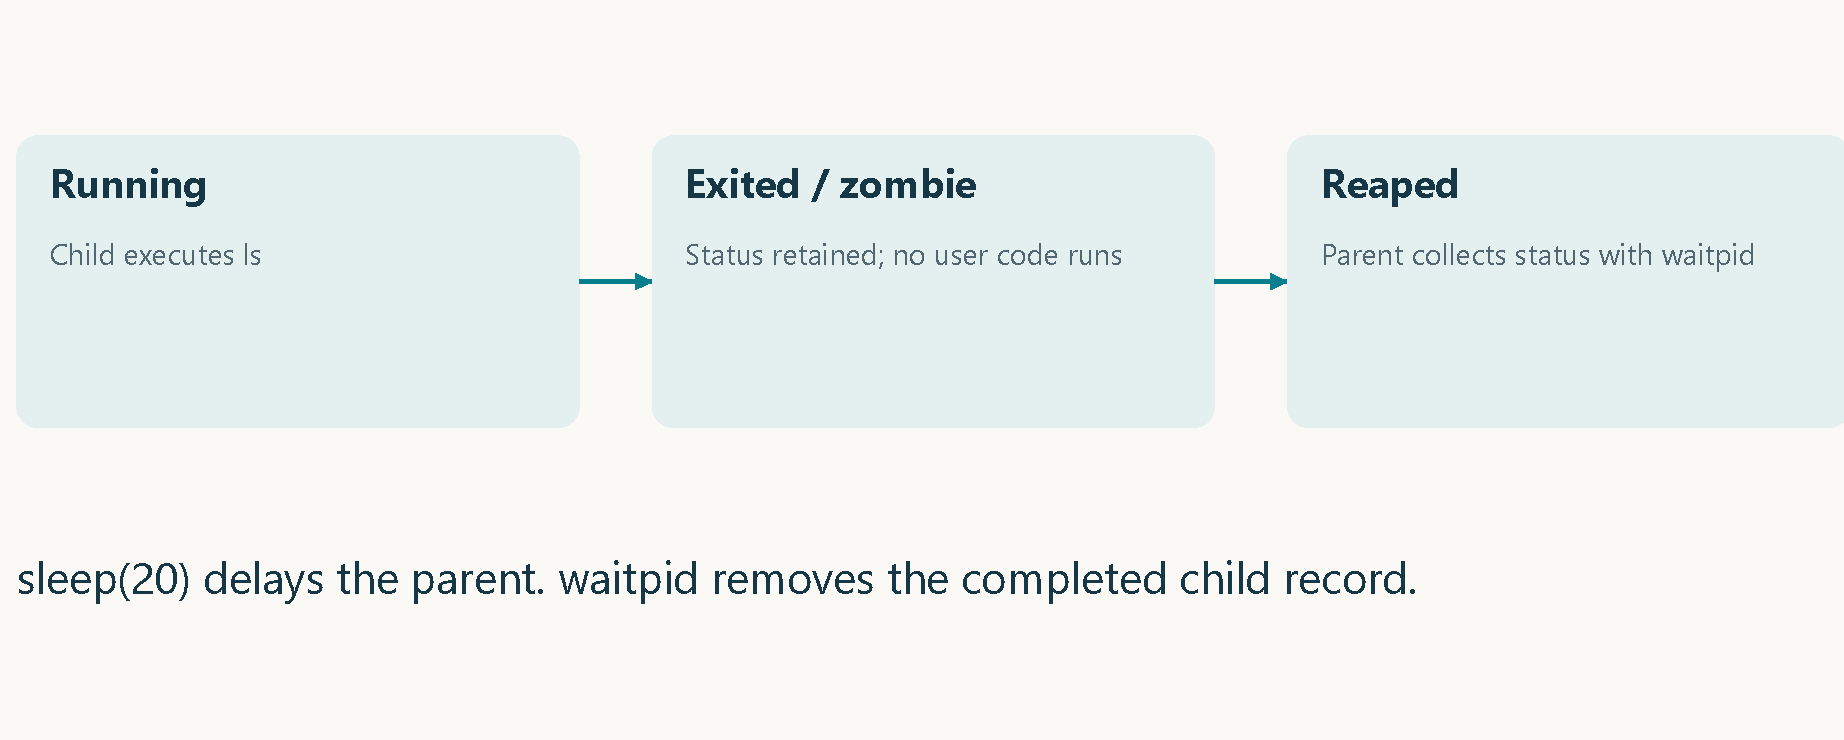
\includegraphics[width=\textwidth]{assets/zombie-lifecycle.pdf}
\caption{An exited child retains an exit record until its parent reaps it.}
\end{figure}


\section{Observe 1}

\textbf{Measured:} While parent PID \texttt{1893} slept, child PID \texttt{1894} had PPID \texttt{1893} and \texttt{STAT} value \texttt{Z+}; \texttt{ps} showed \texttt{[ls] <defunct>}. The \texttt{+} is an additional process-group marker; \texttt{Z} is the zombie state asked about in the brief.


\textbf{Explanation:} \texttt{Z} means the child has exited but its parent has not yet collected its exit status. It is not still executing \texttt{ls}.


\section{Observe 2}

\textbf{Measured:} After the 20-second sleep and \texttt{waitpid}, \texttt{ps} showed no row for parent PID \texttt{1893} or its child.


\textbf{Explanation:} The \texttt{waitpid(pid,\allowbreak{} \&status,\allowbreak{} 0)} at \texttt{zombie.\allowbreak{}c:25} collects the child's remaining exit record. \texttt{sleep(20)} at line 24 only creates time to observe that record.



\begin{figure}[H]
\centering
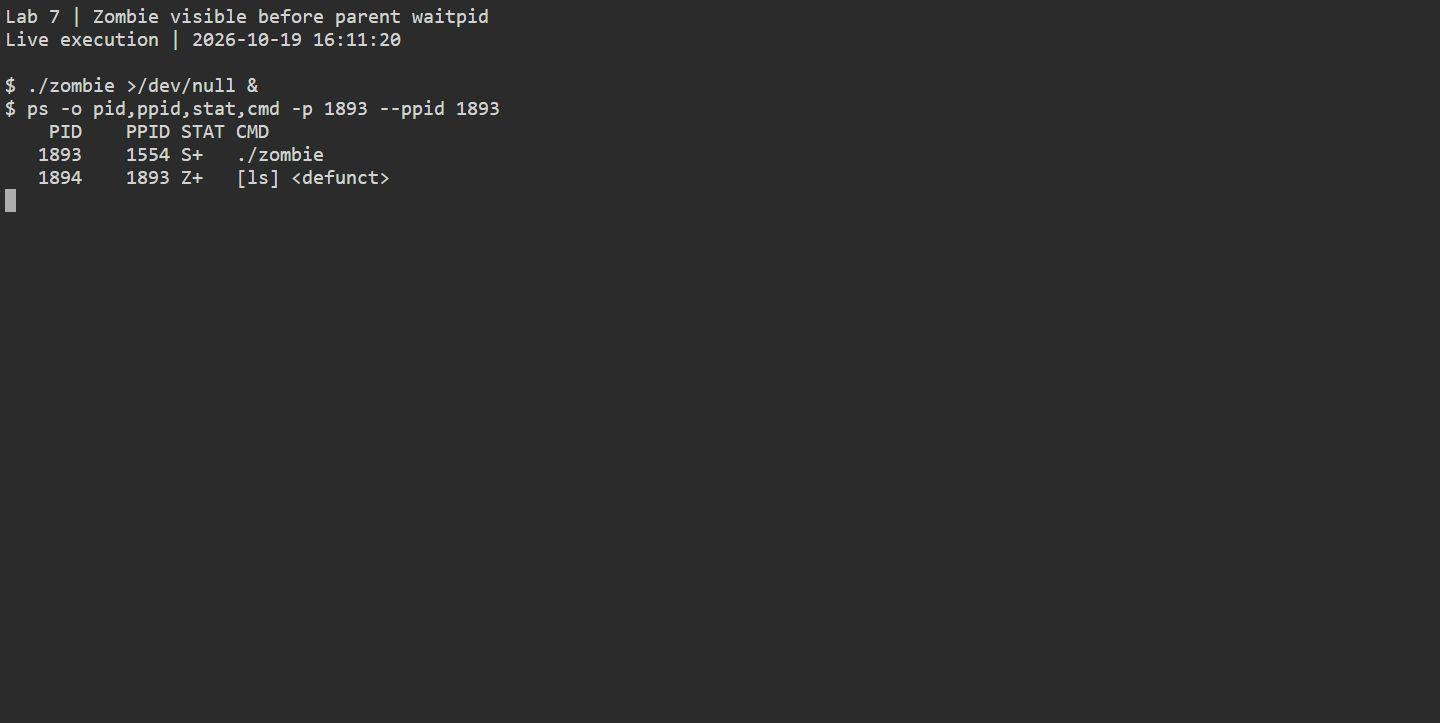
\includegraphics[trim=0bp 493.00bp 320.00bp 0bp,clip,width=\textwidth,height=0.72\textheight,keepaspectratio]{assets/proof-zombie-before.png}
\caption{Before the parent waitpid completes, ps shows the child in zombie state Z. Live ttyd terminal capture, 19 October 2026. Only blank margins are cropped in this report; program output is unchanged.}
\end{figure}


\begin{figure}[H]
\centering
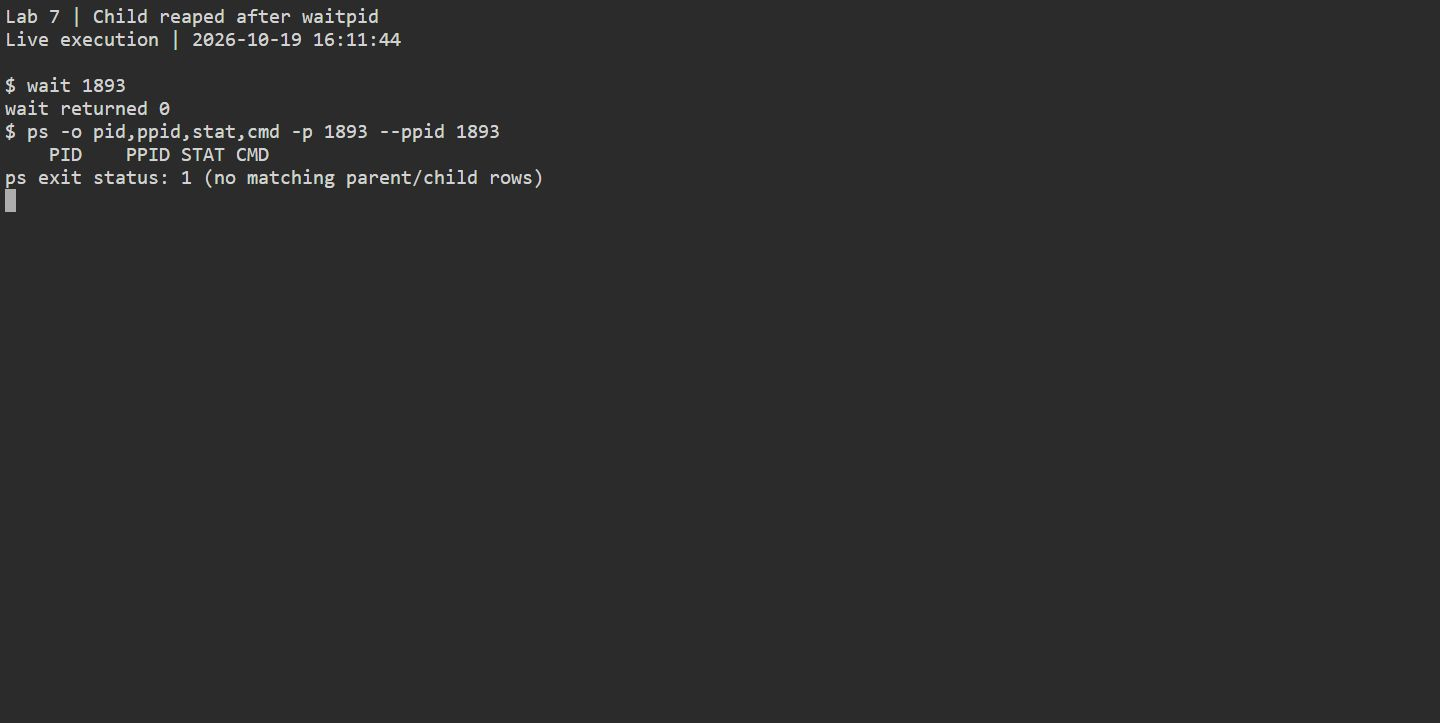
\includegraphics[trim=0bp 493.00bp 320.00bp 0bp,clip,width=\textwidth,height=0.72\textheight,keepaspectratio]{assets/proof-zombie-after.png}
\caption{After waitpid and parent completion, ps no longer finds either of the recorded process rows. Live ttyd terminal capture, 19 October 2026. Only blank margins are cropped in this report; program output is unchanged.}
\end{figure}


\chapter{Part 3: redirection}

A file descriptor is an index in a process's descriptor table, not the file itself. By convention, 0 is standard input, 1 is standard output and 2 is standard error. After \texttt{close(1)}, the lowest free index is 1. Opening \texttt{out.txt} assigns that index to the file. The new program inherits the descriptor connection across \texttt{exec}, so an unchanged \texttt{ls} writes into the file. These changes occur in the child and do not redirect the parent's completion message.


\begin{figure}[htbp]
\centering
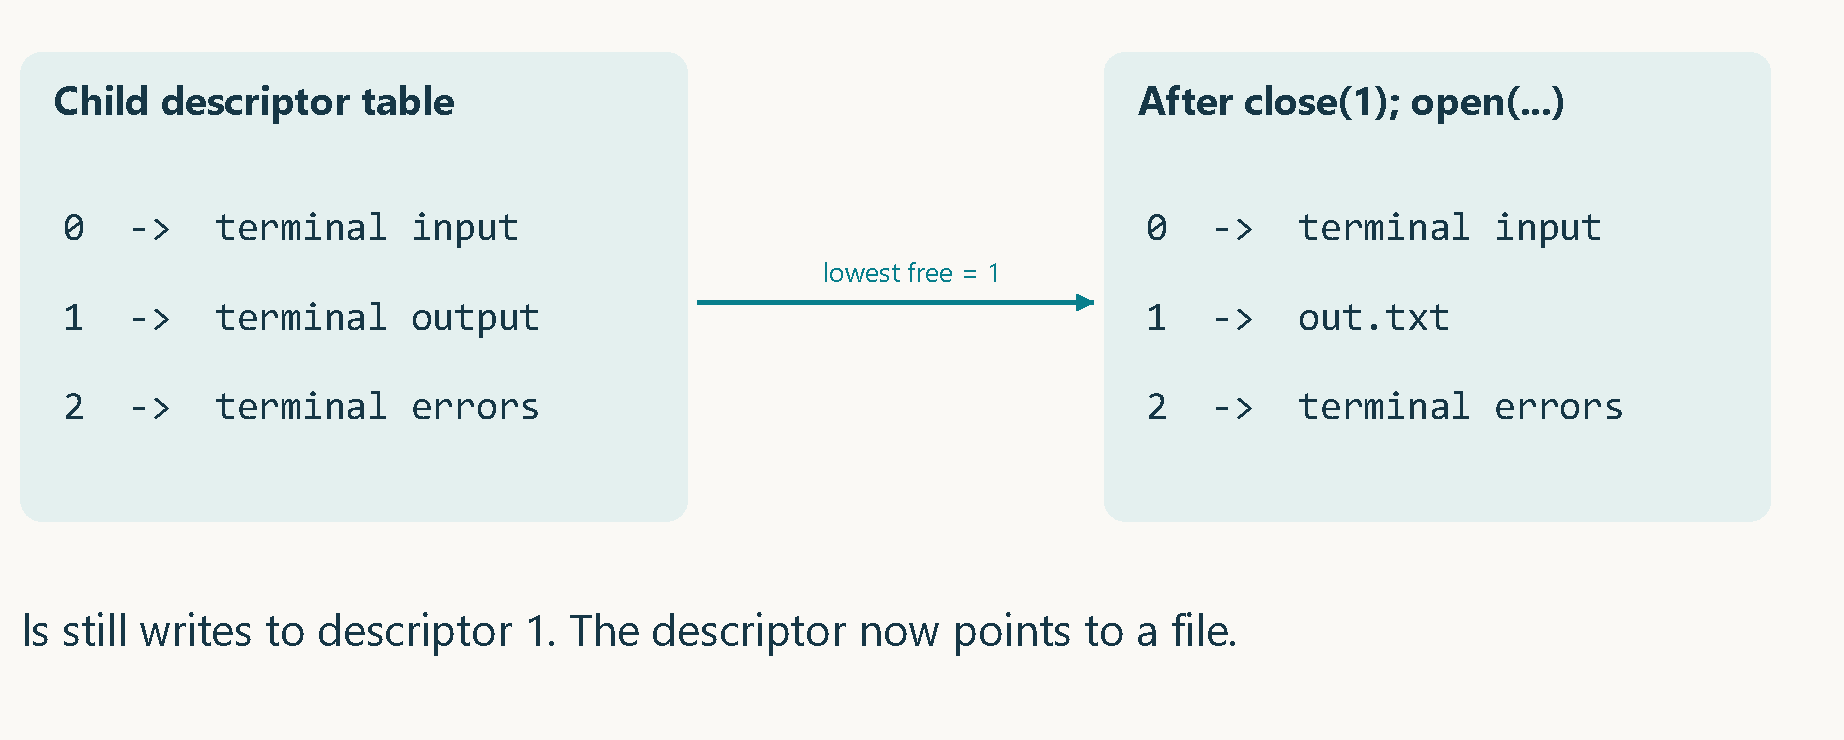
\includegraphics[width=\textwidth]{assets/descriptor-redirection.pdf}
\caption{The child changes descriptor 1 from the terminal to out.txt; descriptor 2 continues to carry diagnostics.}
\end{figure}


\section{Observe 1}

\textbf{Measured:} \texttt{open} reported descriptor \texttt{1}.


\textbf{Explanation:} \texttt{close(1)} frees standard output in the child. \texttt{open} allocates the lowest available descriptor, which is now \texttt{1}.


\section{Observe 2}

\textbf{Measured:} The directory listing was in \texttt{out.\allowbreak{}txt}; the terminal showed the open diagnostic and the parent's completion line.


\textbf{Explanation:} The child uses descriptor \texttt{2} for the diagnostic, so it remains connected to the terminal. After \texttt{open}, descriptor \texttt{1} refers to \texttt{out.\allowbreak{}txt}. \texttt{ls} writes to standard output without knowing that the destination changed.


\section{Observe 3}

To redirect errors like \texttt{2> err.\allowbreak{}txt}, close descriptor \texttt{2} before calling \texttt{open}. Then the file receives the lowest free descriptor, \texttt{2}, which is standard error.



\begin{figure}[H]
\centering
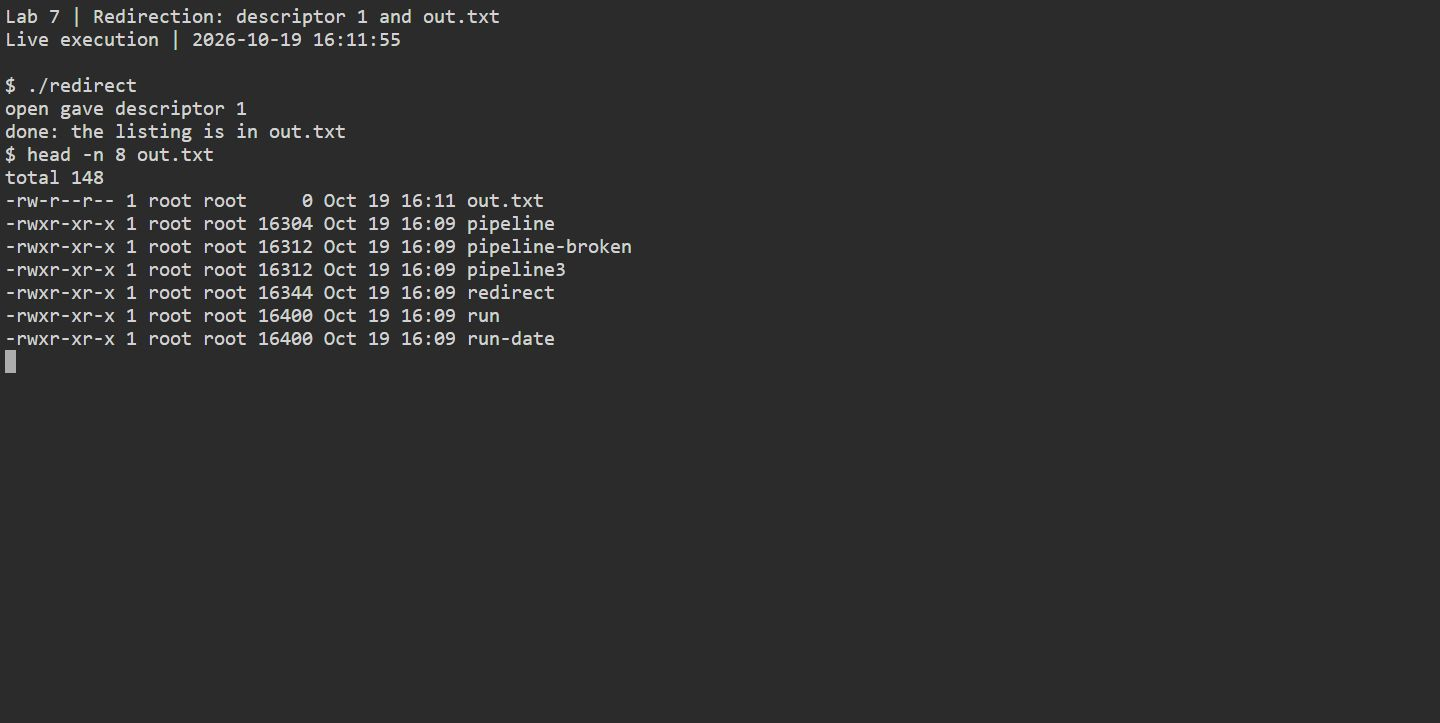
\includegraphics[trim=0bp 332.00bp 320.00bp 0bp,clip,width=\textwidth,height=0.72\textheight,keepaspectratio]{assets/proof-redirection.png}
\caption{open returns descriptor 1; head shows the directory listing stored in out.txt. Live ttyd terminal capture, 19 October 2026. Only blank margins are cropped in this report; program output is unchanged.}
\end{figure}


\chapter{Part 4: a pipe}
Figure~\ref{fig:pipe-eof} shows why closing unused endpoints is part of the algorithm. The two-direction xv6 exchange applies this rule independently to each pipe.

\begin{figure}[htbp]
\centering
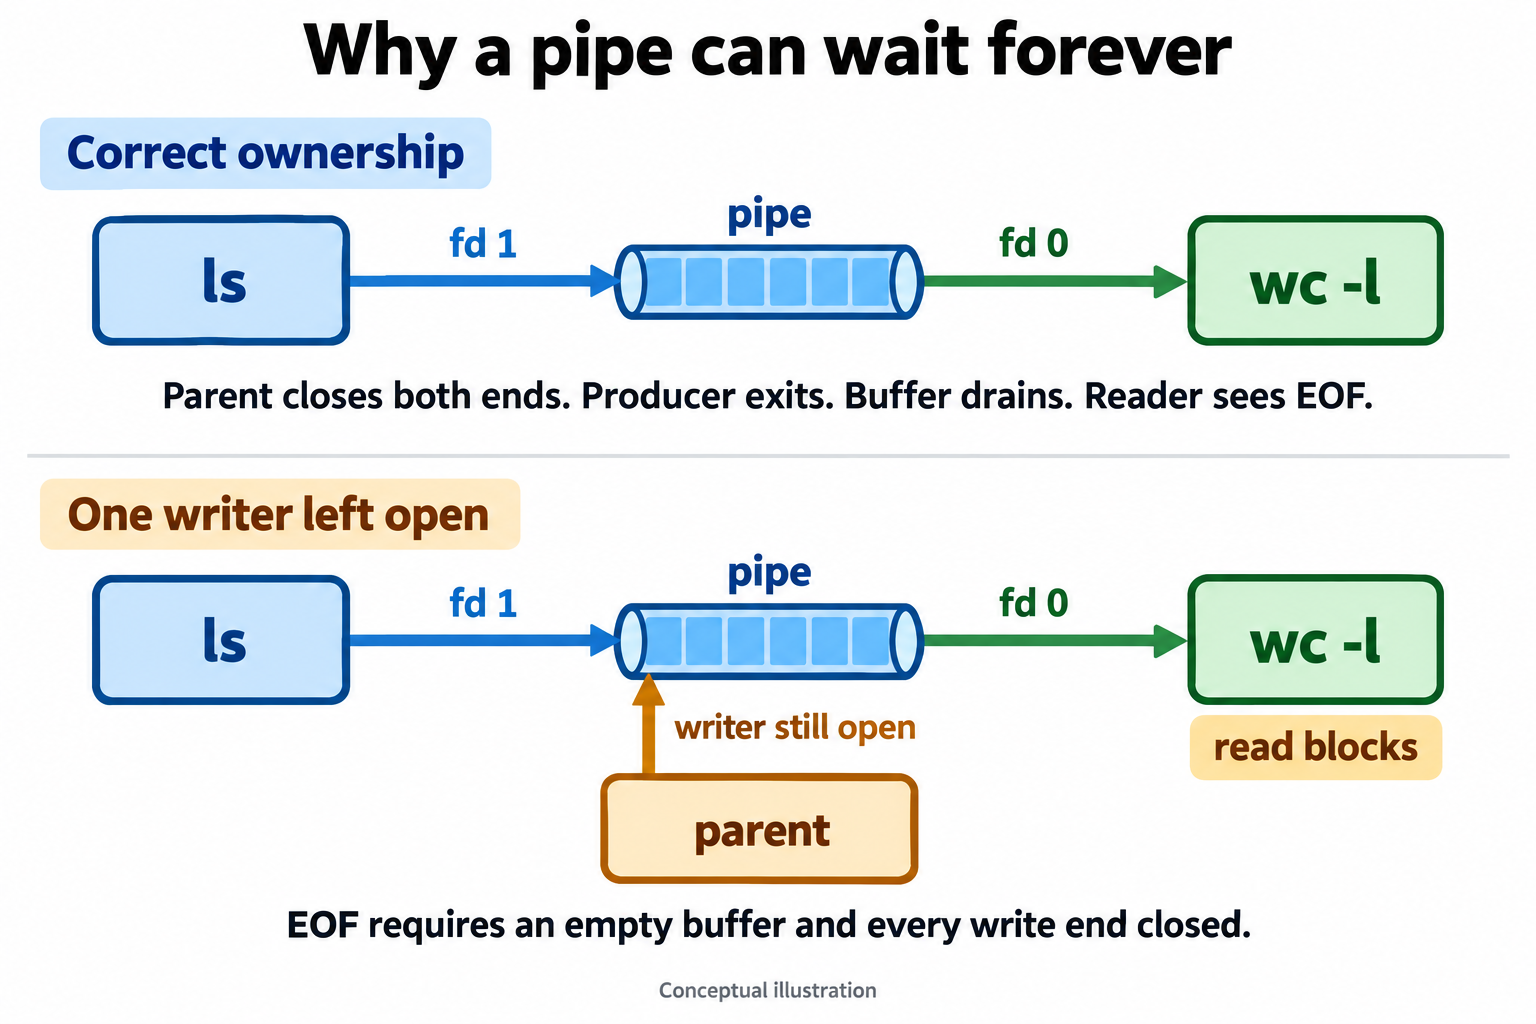
\includegraphics[width=\textwidth]{assets/concept-pipe-ownership.png}
\caption{Writer ownership determines end-of-file. ImageGen concept illustration, 23 October 2026; not measured output.}
\label{fig:pipe-eof}
\end{figure}


\texttt{pipe(p)} creates a byte stream with a read end \texttt{p[0]} and a write end \texttt{p[1]}. Creating it before either fork lets both children inherit references to the same pipe. The producer duplicates the writer onto descriptor 1; the consumer duplicates the reader onto descriptor 0. The original endpoints are then closed in both children, and the parent closes both copies. \texttt{wc -l} counts newline bytes, not structured filesystem entries.

A reader reaches end-of-file only when the buffer is empty and every reference to the write end has closed. If the parent retains its writer, an empty pipe can still receive data, so \texttt{wc} waits. The parent may then wait for \texttt{wc}, exposing the descriptor-lifetime mistake.


\begin{figure}[htbp]
\centering
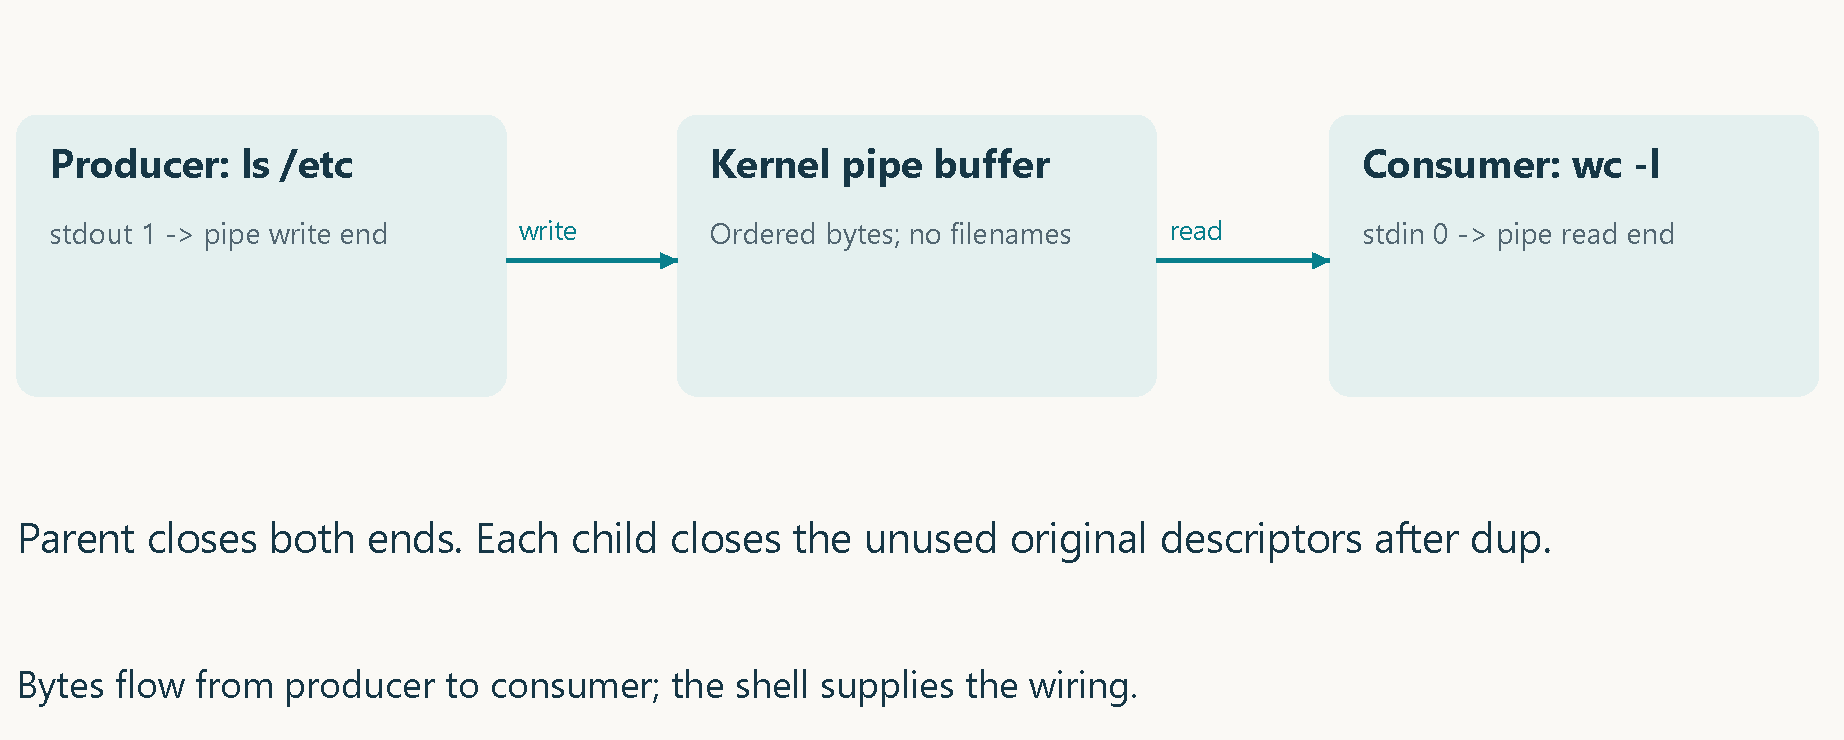
\includegraphics[width=\textwidth]{assets/pipeline-flow.pdf}
\caption{Two child processes connect standard output and standard input through one kernel pipe buffer.}
\end{figure}


\section{Observe 1}

\textbf{Measured:} \texttt{.\allowbreak{}/\allowbreak{}pipeline} printed \texttt{172} and the shell command \texttt{ls /\allowbreak{}etc | wc -\allowbreak{}l} printed \texttt{172} in this run.


\textbf{Explanation:} The first child sends the \texttt{ls /\allowbreak{}etc} listing through the pipe. The second reads that byte stream and counts newline characters with \texttt{wc -\allowbreak{}l}. With the same \texttt{/\allowbreak{}etc} contents, the hand-built pipeline and shell pipeline count the same lines.


\section{Observe 2}

\textbf{Measured:} The intentionally broken variant's parent remained blocked after the bounded 0.5-second wait. The \texttt{ps} snapshot showed \texttt{wc -\allowbreak{}l} PID \texttt{2007} still running with PPID \texttt{2005}, the pipeline parent. The capture runner then sent SIGTERM to the isolated process group \texttt{2005} and waited for the pipeline parent. \texttt{ls} had finished.


\textbf{Explanation:} \texttt{wc} waits for end-of-file. The parent retained a copy of the pipe's write end, so the kernel could not report that all writers were gone even after \texttt{ls} exited.


\section{Observe 3}

\texttt{wc} is waiting for end-of-file on its standard input. End-of-file reaches the reader only after every open reference to the pipe's write end has been closed and the buffered bytes have been consumed.



\begin{figure}[H]
\centering
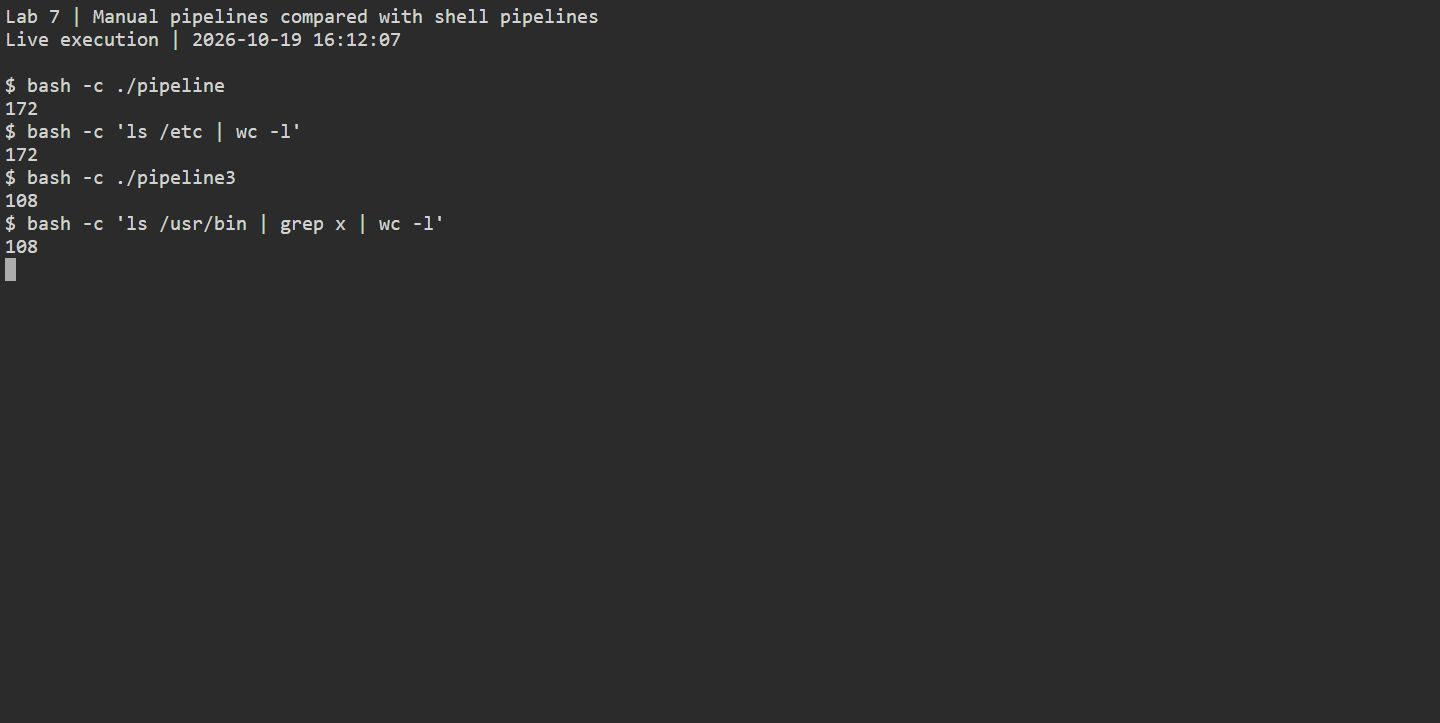
\includegraphics[trim=0bp 424.00bp 320.00bp 0bp,clip,width=\textwidth,height=0.72\textheight,keepaspectratio]{assets/proof-pipelines.png}
\caption{The manual two-stage and optional three-stage pipelines match their shell equivalents. Live ttyd terminal capture, 19 October 2026. Only blank margins are cropped in this report; program output is unchanged.}
\end{figure}


\begin{figure}[H]
\centering
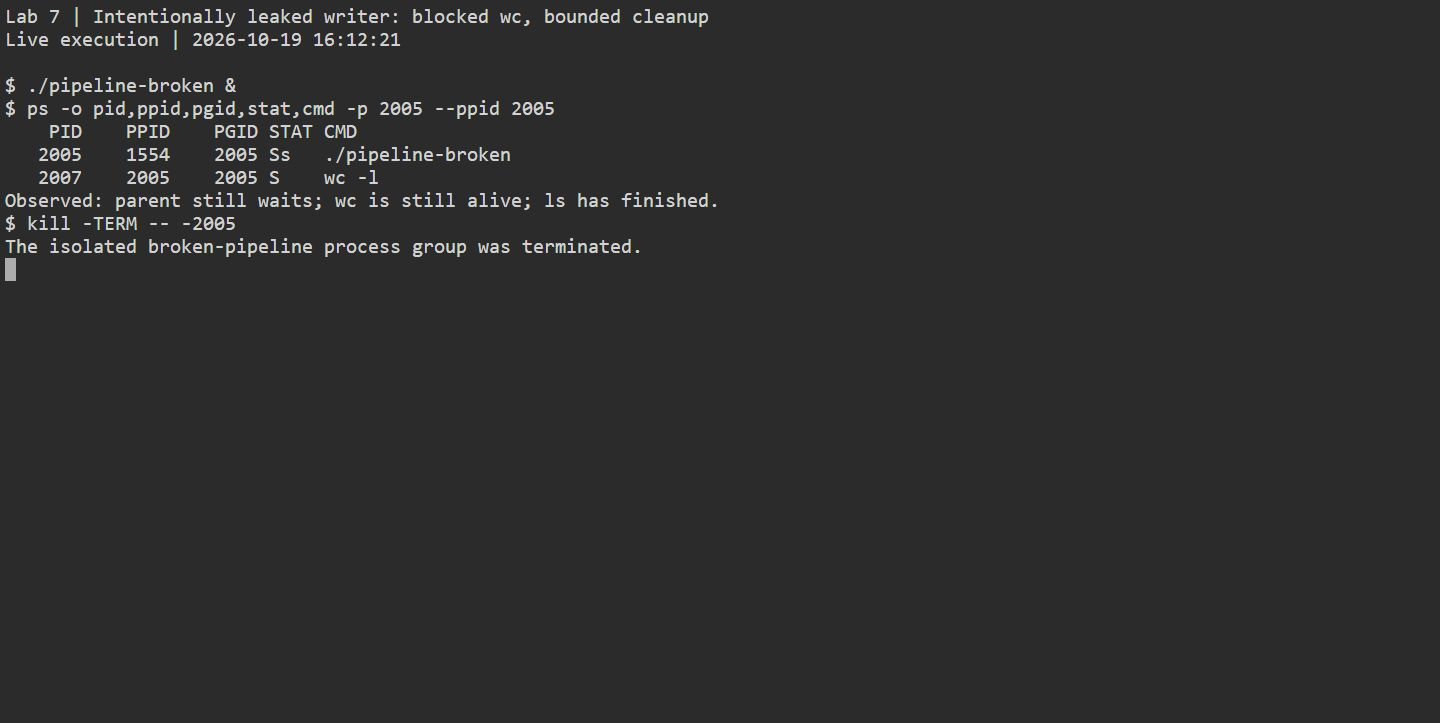
\includegraphics[trim=0bp 424.00bp 320.00bp 0bp,clip,width=\textwidth,height=0.72\textheight,keepaspectratio]{assets/proof-leaked-writer.png}
\caption{With the parent writer deliberately retained, wc remains alive while the parent waits; the isolated group is then stopped. Live ttyd terminal capture, 19 October 2026. Only blank margins are cropped in this report; program output is unchanged.}
\end{figure}


\chapter{Optional three-stage pipeline}

The optional extension uses two pipes and three children. The first pipe carries the directory listing to \texttt{grep x}; the second carries matching lines to \texttt{wc -l}. Each child keeps only its own input and output connections. Closing every unused endpoint allows EOF to propagate through both stages.

\textbf{Measured:} \texttt{pipeline3} printed \texttt{108} and \texttt{ls /\allowbreak{}usr/\allowbreak{}bin | grep x | wc -\allowbreak{}l} printed \texttt{108} in this run.


\textbf{Explanation:} \texttt{ls} writes names to the first pipe, \texttt{grep x} reads those names and writes matching lines to the second pipe, and \texttt{wc -\allowbreak{}l} counts them. All three children and the parent close unused descriptors so each reader can receive end-of-file.


\utmconclusions
The Linux results connect process lifetime to descriptor lifetime. Successful exec replaces the program without creating a new PID; waitpid reaps an exited child. Redirection works by changing descriptor 1 before exec. A pipeline completes when the producer finishes and every writer reference closes, allowing the consumer to observe EOF. Both manual pipelines matched their shell equivalents in the recorded environment.
\begin{thebibliography}{9}
\bibitem{brief} Operating Systems, FCIM/FAF, UTM. \textit{Laboratory 7 handout}, academic year 2026--2027. Accessed 19 October 2026. \url{https://else.fcim.utm.md/mod/resource/view.php?id=72238}.
\bibitem{lecture} Operating Systems. \textit{Processes, Descriptors, Pipes}, Session 4. Accessed 19 October 2026. \url{https://else.fcim.utm.md/mod/resource/view.php?id=72236}.
\bibitem{xv6} MIT. \textit{xv6-riscv source code}. Course source inspected 19 October 2026. Local course snapshot: \texttt{os/lab2}; \texttt{kernel/proc.c}, \texttt{kernel/exec.c}, \texttt{kernel/pipe.c} and \texttt{user/sh.c}.
\end{thebibliography}
\appendix
\chapter{Program source}
The following listings are the submitted programs. They accompany the observations in the main report.


\section{run.c}
\lstinputlisting[language=C]{run.c}

\section{zombie.c}
\lstinputlisting[language=C]{zombie.c}

\section{redirect.c}
\lstinputlisting[language=C]{redirect.c}

\section{pipeline.c}
\lstinputlisting[language=C]{pipeline.c}

\section{pipeline3.c}
\lstinputlisting[language=C]{pipeline3.c}

\end{document}
